\documentclass[final]{beamer}\usepackage[]{graphicx}\usepackage[]{color}
%% maxwidth is the original width if it is less than linewidth
%% otherwise use linewidth (to make sure the graphics do not exceed the margin)
\makeatletter
\def\maxwidth{ %
  \ifdim\Gin@nat@width>\linewidth
    \linewidth
  \else
    \Gin@nat@width
  \fi
}
\makeatother

\definecolor{fgcolor}{rgb}{0.345, 0.345, 0.345}
\newcommand{\hlnum}[1]{\textcolor[rgb]{0.686,0.059,0.569}{#1}}%
\newcommand{\hlstr}[1]{\textcolor[rgb]{0.192,0.494,0.8}{#1}}%
\newcommand{\hlcom}[1]{\textcolor[rgb]{0.678,0.584,0.686}{\textit{#1}}}%
\newcommand{\hlopt}[1]{\textcolor[rgb]{0,0,0}{#1}}%
\newcommand{\hlstd}[1]{\textcolor[rgb]{0.345,0.345,0.345}{#1}}%
\newcommand{\hlkwa}[1]{\textcolor[rgb]{0.161,0.373,0.58}{\textbf{#1}}}%
\newcommand{\hlkwb}[1]{\textcolor[rgb]{0.69,0.353,0.396}{#1}}%
\newcommand{\hlkwc}[1]{\textcolor[rgb]{0.333,0.667,0.333}{#1}}%
\newcommand{\hlkwd}[1]{\textcolor[rgb]{0.737,0.353,0.396}{\textbf{#1}}}%
\let\hlipl\hlkwb

\usepackage{framed}
\makeatletter
\newenvironment{kframe}{%
 \def\at@end@of@kframe{}%
 \ifinner\ifhmode%
  \def\at@end@of@kframe{\end{minipage}}%
  \begin{minipage}{\columnwidth}%
 \fi\fi%
 \def\FrameCommand##1{\hskip\@totalleftmargin \hskip-\fboxsep
 \colorbox{shadecolor}{##1}\hskip-\fboxsep
     % There is no \\@totalrightmargin, so:
     \hskip-\linewidth \hskip-\@totalleftmargin \hskip\columnwidth}%
 \MakeFramed {\advance\hsize-\width
   \@totalleftmargin\z@ \linewidth\hsize
   \@setminipage}}%
 {\par\unskip\endMakeFramed%
 \at@end@of@kframe}
\makeatother

\definecolor{shadecolor}{rgb}{.97, .97, .97}
\definecolor{messagecolor}{rgb}{0, 0, 0}
\definecolor{warningcolor}{rgb}{1, 0, 1}
\definecolor{errorcolor}{rgb}{1, 0, 0}
\newenvironment{knitrout}{}{} % an empty environment to be redefined in TeX

\usepackage{alltt}
\usepackage{grffile}
\mode<presentation>{\usetheme{CambridgeUSPOL}}

\usepackage[utf8]{inputenc}
\usepackage{amsfonts}
\usepackage{amsmath}
\usepackage{natbib}
\usepackage{graphicx}
\usepackage{array,booktabs,tabularx}
\usepackage{epstopdf}
\usepackage{colortbl, xcolor}
\newcolumntype{Z}{>{\centering\arraybackslash}X}

% rysunki
\usepackage{tikz}
\usepackage{ifthen}
\usepackage{xxcolor}
\usetikzlibrary{arrows}
\usetikzlibrary[topaths]
\usetikzlibrary{decorations.pathreplacing}
%\usepackage{times}\usefonttheme{professionalfonts}  % times is obsolete
\usefonttheme[onlymath]{serif}
\boldmath
\usepackage[orientation=portrait,size=a0,scale=1.4,debug]{beamerposter}                       % e.g. for DIN-A0 poster
%\usepackage[orientation=portrait,size=a1,scale=1.4,grid,debug]{beamerposter}                  % e.g. for DIN-A1 poster, with optional grid and debug output
%\usepackage[size=custom,width=200,height=120,scale=2,debug]{beamerposter}                     % e.g. for custom size poster
%\usepackage[orientation=portrait,size=a0,scale=1.0,printer=rwth-glossy-uv.df]{beamerposter}   % e.g. for DIN-A0 poster with rwth-glossy-uv printer check
% ...
%

\usecolortheme{seagull}
\useinnertheme{rectangles}
\setbeamercolor{item projected}{bg=darkred}
% \setbeamertemplate{enumerate items}[default]
\setbeamertemplate{caption}{\insertcaption} 
\setbeamertemplate{navigation symbols}{}
\setbeamercovered{transparent}
\setbeamercolor{block title}{fg=darkred}
\setbeamercolor{local structure}{fg=darkred}

\setbeamercolor*{enumerate item}{fg=darkred}
\setbeamercolor*{enumerate subitem}{fg=darkred}
\setbeamercolor*{enumerate subsubitem}{fg=darkred}

%\setbeamercolor*{itemize item}{fg=darkred}
%\setbeamercolor*{itemize subitem}{fg=darkred}
%\setbeamercolor*{itemize subsubitem}{fg=darkred}

\newlength{\columnheight}
\setlength{\columnheight}{96.5cm}
\renewcommand{\thetable}{}
\def\andname{,}
\authornote{}

\renewcommand{\APACrefatitle}[2]{}
\renewcommand{\bibliographytypesize}{\footnotesize} 
\renewcommand{\APACrefYearMonthDay}[3]{%
  {\BBOP}{#1}
  {\BBCP}
}
\IfFileExists{upquote.sty}{\usepackage{upquote}}{}
\begin{document}


\date{}

\author{\large \underline{Jaros\l{}aw Chilimoniuk}\inst{1}, Pawe\l{} Mackiewicz\inst{1} and Micha\l{} Burdukiewicz\inst{2}*\\
\bigskip
\normaltext{*jaroslaw.chilimoniuk@gmail.com}}

\institute{\small{\textsuperscript{1}University of Wroc\l{}aw, Department of Genomics, Wroc\l{}aw, POLAND
\textsuperscript{2}Warsaw University of Technology, Warsaw, POLAND}}

\title{\huge CsgA, CsgB and CsgC - evolutionary interplay in curli biogenesis}

\begin{frame}
\begin{columns}
\begin{column}{.50\textwidth}
\begin{beamercolorbox}[center,wd=\textwidth]{postercolumn}
\begin{minipage}[T]{.95\textwidth}
\parbox[t][\columnheight]{\textwidth}
{
\begin{block}{Introduction}


  

CsgA, also known as a major curli component, is a secreted protein ubiquitous in biofilms of gram-negative bacteria (Zhou et al., 2012a). Thanks to its ability to create durable fibers, CsgA is a dominant proteinaceous scaffold of biofilms. In fact, CsgA belongs to amyloids, proteins that form fibers during a spontaneous aggregation. CsgC, a sequence-specific inhibitor, is able to arrest aggregation of CsgA in periplasmic space (Evans et al., 2015).

The presence of pre-formed amyloid fibers can accelerate aggregation of other amyloids. This process is known as cross-seeding. It is extremely sequence specific and can be restricted by a difference in a single amino acid (Zhou et al., 2012b). CsgA can be in vivo cross-seeded by its nucleator protein, CsgB, but also other CsgA fibrils.
\end{block}


  \begin{block}{Methods}
  We recently published AmyloGram (Burdukiewicz et al., 2017). It is an efficient tool for prediction of amyloid proteins as CsgA and CsgB. Among others, our algorithm produces a simplified amino acid alphabet for amyloid proteins. It groups amino acid together into six groups based on their physicochemical features. We combined sequences of around 500 triplets CsgA-CsgB-CsgC from closely related gram-negative bacteria and used EVmutation software (Hopf et al., 2017) to find out which residues are especially susceptible to simultaneous mutations. 
\end{block}


  \begin{block}{Results}


\begin{knitrout}
\definecolor{shadecolor}{rgb}{0.969, 0.969, 0.969}\color{fgcolor}

{\centering 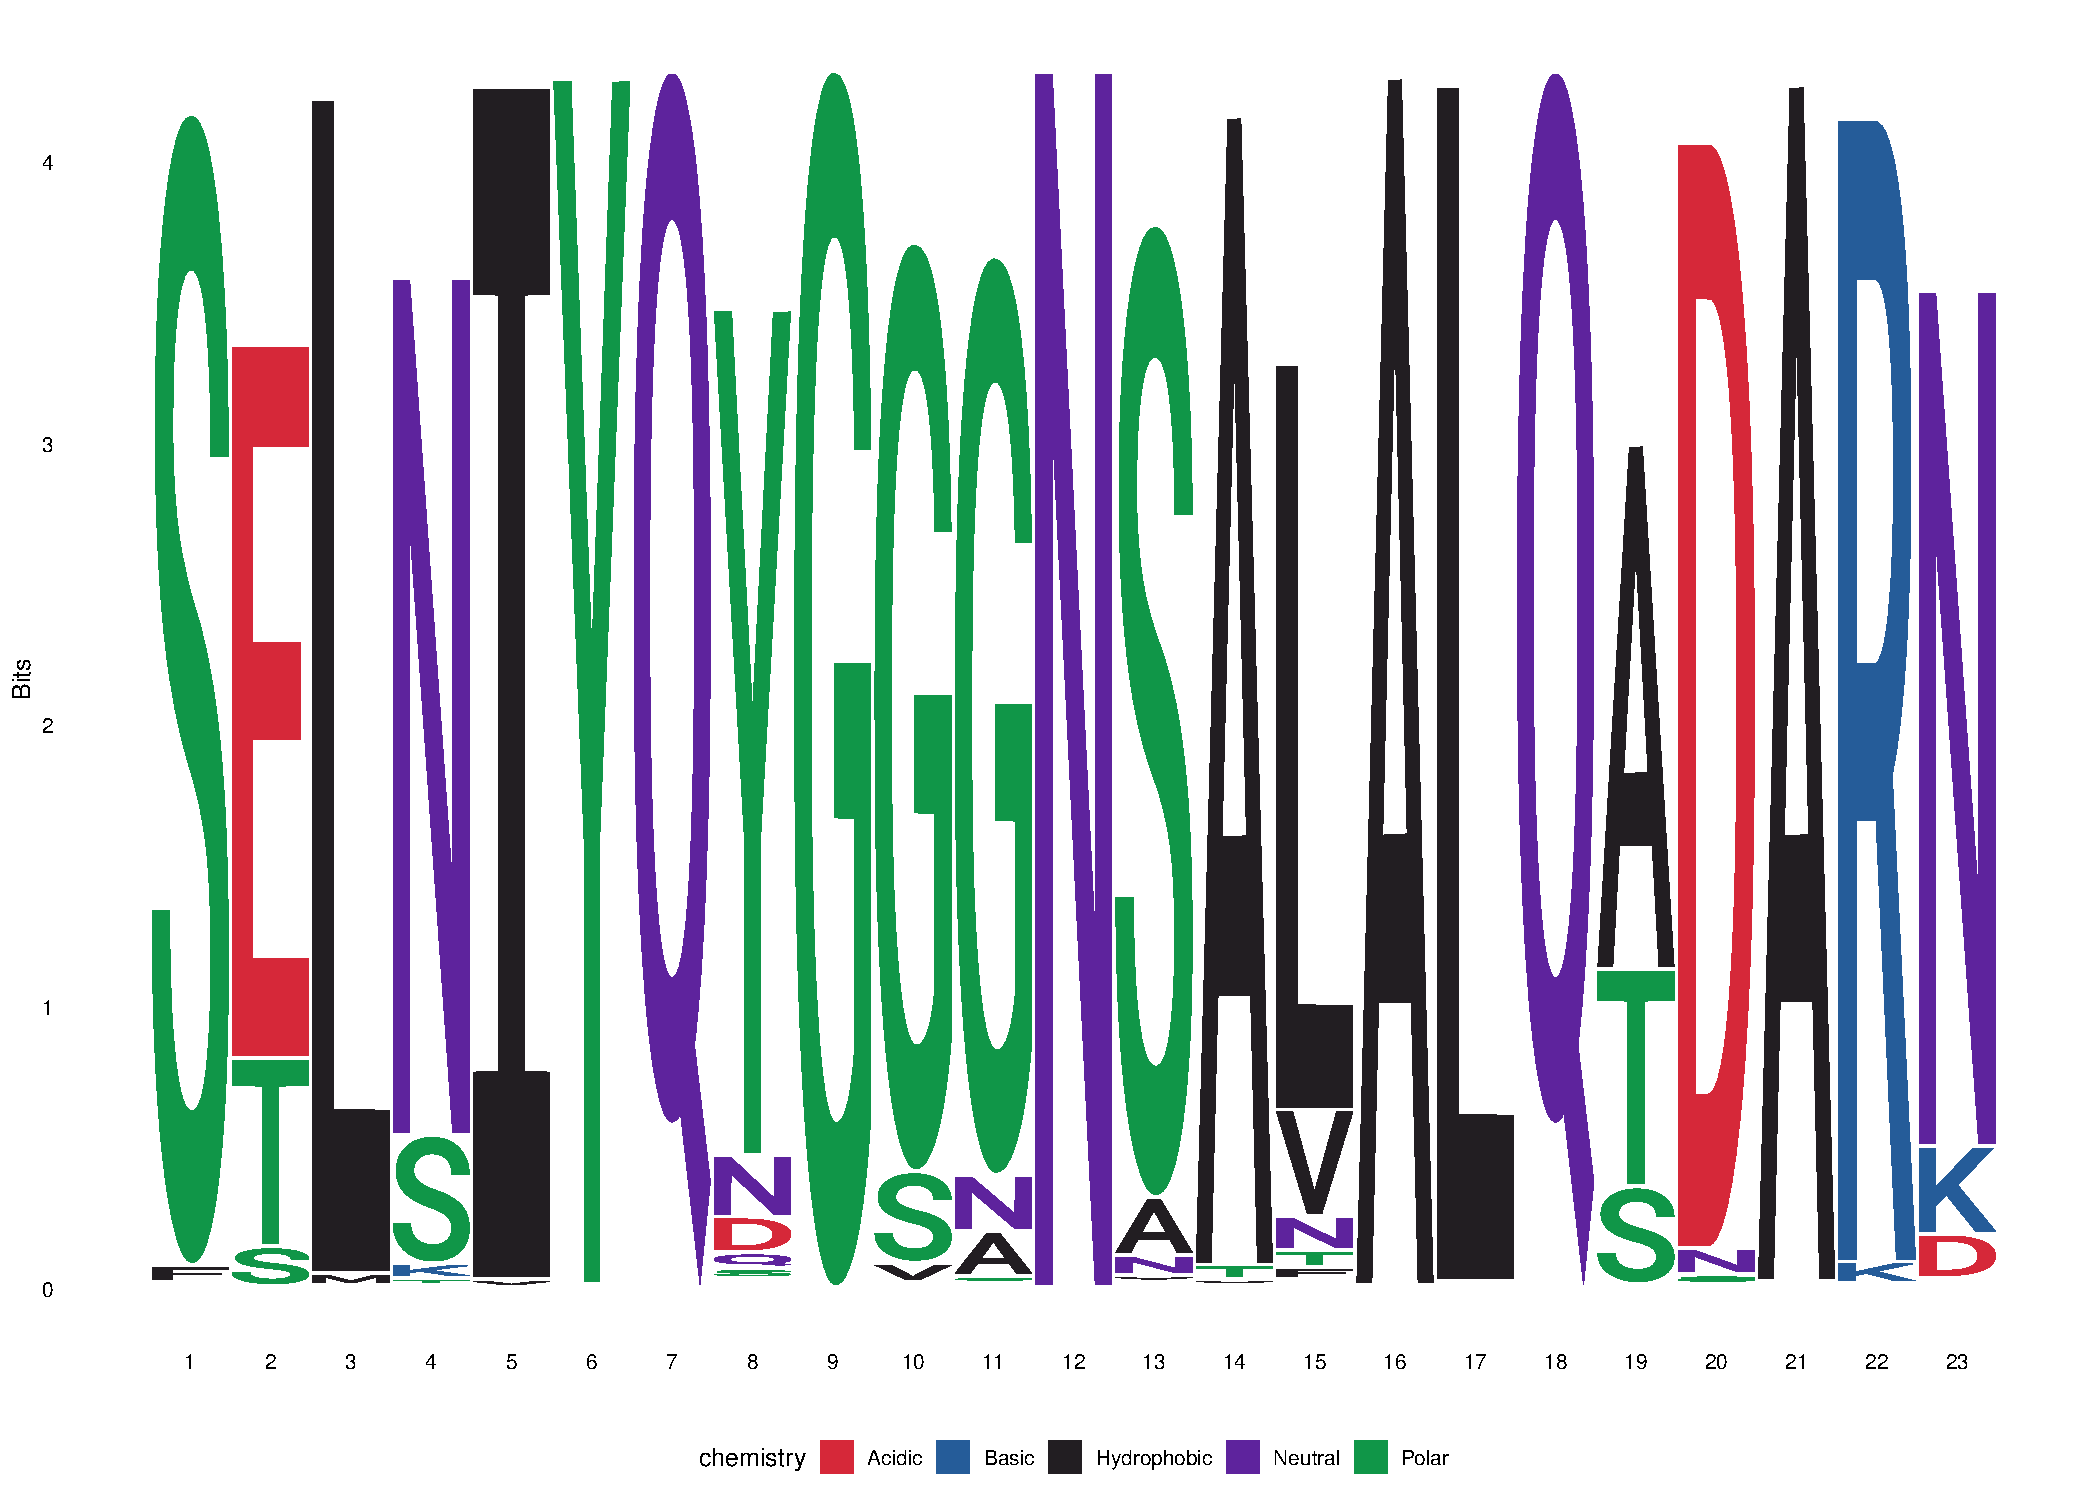
\includegraphics[width=\maxwidth]{figure/unnamed-chunk-1-1} 

}



\end{knitrout}
  

Both CsgA and CsgB are characterized by a regional structure of five repeated motifs. We found out that the general motif (S-X5-Q-X-G-X2-N-X-A-X3-Q) (the serin in absent in the case of CsgB) is faithfully preserved among different variants of CsgA and CsgB. The residual variability in motifs of both proteins does not affect the sequence of other protein.

The opposite situation happens in CsgC, where mutations are not limited to specific motifs. On the other hand, CsgA and CsgC keep a similar level of the sequence divergence aside from species of Enterobacter and Salmonella genera, where CsgC accumulates more mutations.


    \end{block}
    \vfill
}
\end{minipage}
\end{beamercolorbox}
\end{column}


%new column ------------------------------------------------------    

\begin{column}{.51\textwidth}
\begin{beamercolorbox}[center,wd=\textwidth]{postercolumn}
\begin{minipage}[T]{.95\textwidth}  
\parbox[t][\columnheight]{\textwidth}
{


    \begin{block}{Conclusions}
      
      
      The interplay of CsgA, CsgB and CsgC suggests that if a mutation occurs in the region responsible for protein interaction, it should be compensated by mutations in other two proteins. For example, the presence of mutations that decrease the aggregation rate of CsgA, allows CsgC to become a less effective inhibitor without affecting the wellbeing of bacteria. Our preliminary study partially confirms this hypothesis by finding out that genera with less efficient CsgA, as Salmonella, can accumulate more mutations in the sequence of CsgC.

We have not identified any simultaneous mutations between CsgA and CsgB. This may be due that single mutation in one region is not enough to change the protein function and to cause mutations in another protein. Probably, the compensation of single mutations by the regional structure of mentioned proteins is sufficient.

    \end{block}
    \vfill 
    

}
\end{minipage}
\end{beamercolorbox}
\end{column}
\end{columns}  
\end{frame}
\end{document}
